\chapter{Theory}
\section{Machine Learning}

Historically computers had to be programmed on a specific task using domain knowledge of humans. Machine learning challenges this traditional way of programming. Rather than trough extensive domain knowledge, machine learning algorithms are used to autonomously learn from data and information. 
\\
%https://www.forbes.com/sites/bernardmarr/2016/02/19/a-short-history-of-machine-learning-every-manager-should-read/#77bf286315e7

This intention is often represented by a 'learning' \emph{input-output function}. Assume there exists function, $f$, which represents a true behaviour or correlation. The task of any machine learning algorithm is thereby to find a \emph{hypothesis function} $h$ that resembles the behaviour of $f$ as closely as possible. A function $h$ is also called \emph{model}. Both $f$ and $h$ are function of a fixed length vector-valued input $X={x_1, x_2, ... , x_n}$ which has $n$ components. Those might be $n$ attributes of an observed object. An input $x$ is often referred to as a \emph{data point}. The components of a data point $x$ are the \emph{features} of $x$. 
The features of a data point span the \emph{feature space}. The feature space refers to the $n$-dimensional space in which the features of a data point are represented.
\\
The function $h$ can be thought of as a device that has $X$ as an input and $h(X)$ as an output. The hypothesis function, h, is selected based on a trainings set, $\Xi$, of $m$ input vector examples.
\\
There are two major settings in machine learning. 
\\
The first setting is \emph{unsupervised learning}. In this case the trainings set of vectors $\Xi$ doesn't provide information about the value $f(X)$ . The goal of the unsupervised learning algorithms usually is to partition the training set into subset, $\Xi$ \textsubscript{1}, $\Xi$ \textsubscript{2}, ..., $\Xi$ \textsubscript{r}. An example for unsupervised machine learning learning is \emph{clustering}, which finds clusters and discovers relationships in the data.
\\
The second is  \emph{supervised learning}, in which the values of $f$ for the samples in the training set $\Xi$ are known. The value of $f$ corresponding to a data point $x$ is also called the \emph{label} of $x$. A dataset with a label for every data point in it is referred to as a \emph{labelled} dataset. The assumption is that a hypothesis $h$ is a good guess for $f$ when $h(x_i)$ agrees with the values of $f(x_i)$ or the given labels for the majority of samples $x_i$ .
%classification application in pattern recognition 
% http://cs.du.edu/~mitchell/mario_books/Introduction_to_Machine_Learning_-_2e_-_Ethem_Alpaydin.pdf 6
\\
In supervised machine learning two main areas are distinguished, \emph{Regression} and \emph{Classification}. 
\\
In Regression the hypothesis $h$ has a continuous output. Regression could, for instance, be used to approximate a function for a stock price and predict a future stock price as a numerical value on a continuous range of possible prices.
\\
Classification has a categorical output. Classification could, for instance, be used to classify emails to either spam or no spam. It also finds application in patter recognition. % http://cs.du.edu/~mitchell/mario_books/Introduction_to_Machine_Learning_-_2e_-_Ethem_Alpaydin.pdf 6? 
The case of an classification task that has a need to classify data into two distinguished classes is called \emph{binary classification}. The alternative case is \emph{multiclass classification}, which aims to classify data points into one of multiple different classes.

%classification, inpu, representation, hypotesis, generalization:
% http://cs.du.edu/~mitchell/mario_books/Introduction_to_Machine_Learning_-_2e_-_Ethem_Alpaydin.pdf 21

\section{Evaluation of Classifiers}
\begin{itemize}
\item{f-score}
fscore , precision, recall
% http://delivery.acm.org/10.1145/320000/312647/p42-yang.pdf?ip=134.155.178.109&id=312647&acc=ACTIVE%20SERVICE&key=2BA2C432AB83DA15%2E33B98ACB330D6FA0%2E4D4702B0C3E38B35%2E4D4702B0C3E38B35&CFID=976370719&CFTOKEN=43508633&__acm__=1503605339_b0f297be35db501d0410685c60e0b4b6
(2 oben rechts)
\item{Cross validation}
% https://wiki.eecs.yorku.ca/course_archive/2014-15/F/4412/_media/ensemble_data_mining.pdf 26 (44)

especially k-fold validation: 
is non exhaustive

% http://ai.stanford.edu/people/nilsson/MLBOOK.pdf  82

\end{itemize}
\section{Algorithms}
\begin{itemize}
\item{hyper-parameters}
\item{loss function / regularization}
\item{varance/over/underfitting}
\item{linear/non linear}
\item{may be oversimplyfied because of rahmen der arbeit}
% http://jmlr.csail.mit.edu/papers/volume13/bergstra12a/bergstra12a.pdf 2
\end{itemize}
\subsection{Linear support vector classifier}
In this chapter the support vector classifier will be introduced. The method was developed in the 1990’s and is often used as one of the best performing 'out of the box' classifiers. The goal of a linear support classifier is to find a function for a \emph{hyperplane} that splits the data points of two classes as best as possible. The support vector classifier is a extension of a maximal margin classifier. First  the concept of classification using a hyperplane and with a maximal margin classifier will be explained. Then the extension to a support vector classifier will be shown.
A model based on a support vector classifier is linear.
\subsubsection{Hyperplane classification}
The goal of the maximal margin classifier is to classify data by finding a hyperplane that optimally separates two classes in a dataset. Data points are either in class $y=f(x)=-1)$ or $y=f(x)=1)$. 
\\
A hyperplane is a flat affine subspace of dimension $p-1$, where p is the number of dimensions the hyperplane is in. In the case of a maximal margin classifier the number of dimensions which a hyperplane will be constructed in is the number dimension of the feature space. This stems from the intention to separate data points which have a feature vector of $p$ dimensions. Accordingly a hyperplane is defined by
\begin{equation} \label{eq:1}
\beta_0 + \beta_1 X_1 + ... + \beta_p X_p = 0
\end{equation}
for a feature space of dimension p. It can be said that $\beta_0$  to $\beta_p$ 'define' the hyperplane.
If a point $X=(x_1,x_2,...,x_p)$ lies on the hyperplane, the point features $x_1$ to $x_p$ would satisfy the equation \ref{eq:1}.
\\
If this doesn't hold true but
\begin{equation} \label{eq:2}
\beta _0 + \beta _1 X_1 + ... + \beta_p X_p > 0
\end{equation}
is true, the point $X$ lies on the one side of the plane, whereas if 
\begin{equation} \label{eq:3}
\beta_0 + \beta_1 X_1 + ... + \beta_p X_p < 0
\end{equation}
is true, the the point $X$ lies on the other side. 
\\
If a hyperplane is defined in a way that the data points of on class lay on the one side of the hyperplane and the data points of the other class on the other side, any given data point can be classified accordingly as either one or the other class according to equations \ref{eq:2} and \ref{eq:3}.
\\
The \emph{magnitude} of $h(X)$ can be used to derive a confidence score for the classification. A higher magnitude of $h(X)$, which can be interpreted as distance to the plane, corresponds to a higher confidence in the classification.


\subsubsection{Maximal margin classifier}

If a class separating hyperplane exist there exists an infinite number of such hyperplanes separating the classes (a hyperplane can always be moved or varied slightly while still remaining class separating). The question arises which hyperplane should be used. 
\\
A maximal margin classifier uses the hyperplane, where the distance to the next data point  is the biggest under all possibilities. The distance to the next data point is called the \emph{margin}. A hyperplane that has the biggest possible margin is a \emph{maximal margin hyperplane}. Data points where the distance to the maximal margin hyperplane is equal to the margin are the \emph{support vectors} as seen in figure \ref{fig:mmh}. The maximal margin hyperplane depends on the support vectors because moving or removing the support vectors would change the hyperplane. Moreover the vectors that are further away from the hyperplane than the support vectors don't contribute to definition of the hyperplane. This allows the hyperplane to be soly defined by the support vectors.\\

\begin{figure}[h]
\centering
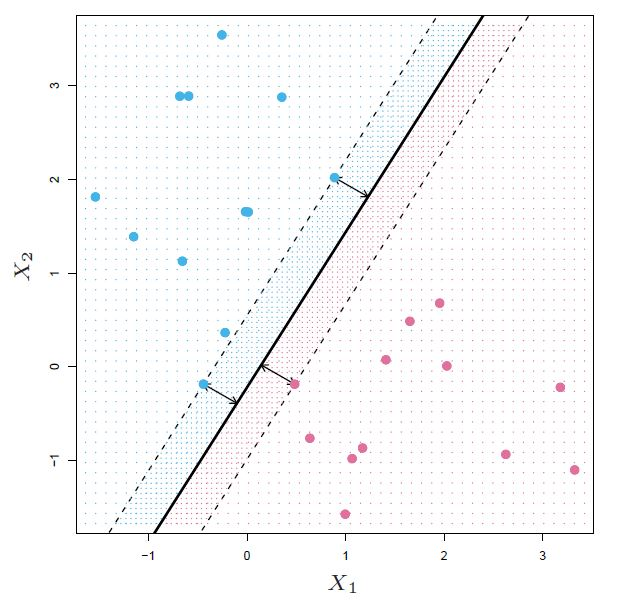
\includegraphics[width=0.7\textwidth]{PE4/svm.JPG}
\caption{Maximal margin hyperplane separating two classes of data points with the margin borders visualized by dotted lines}
\label{fig:mmh}
\end{figure}

To find a maximal margin hyperplane the parameters of the hyperplane have to be set in a way that maximises the size of the margin $M$ and
\begin{equation} \label{eq:7}
y_i(\beta_0+beta_1 x_i1 +\beta_2 x_i2 + ... +\beta_p x_ip) \leq M   \forall i=1,...,n
\end{equation}
holds.
$y_i$ is the true class of the $i$th data point. If all data points are classified correctly, which is the goal, the left side of the equation \ref{eq:7} is always positive. This is because either both $y_i$ and $f(X_i)$ are negative or both are positive. The right side of the equation makes sure that every data point has a minimal distance of M to the hyperplane.

The maximal margin classifier has some faults that have to be considered. Because the data points are of a class are strictly separated by a hyperplane of a linear form from the other class, it is not possible to find a hyperplane if the classes are not linear separable.  Furthermore even when the classes are linear separable the hyperplane pound might be forced in a unfavourable spot by only one single data point that doesn't represent most of the other data points of the same class. The extension to a support vector classifier solves those problems.

\subsubsection{Support vector classifier}

To solve the above mentioned faults the \emph{support vector classifier}, also called \emph{soft margin classifier}, allows some data points of the training data to be not on the correct side of the margin or the hyperplane. 
\\
To find a hyperplane for a support vector classifier the parameters of the hyperplane have to be set in a way that maximises the size of the margin $M$ and the equations 
\begin{equation} \label{eq:8}
y_i(\beta_0+beta_1 x_i1 +\beta_2 x_i2 + ... +\beta_p x_ip) \leq M(1- \epsilon_i ) \forall i=1,...,n
\end{equation}

\begin{equation} \label{eq:9}
\epsilon_i >= 0, \sum_i=1^n \epsilon_i \leq	 C
\end{equation}

both hold.\\
The concept is similar to the one seen in equation \ref{eq:7}. Differentiating here are the \emph{slack variables} $\epsilon_1, ..., \epsilon_n$. $\epsilon_i$ indicates where the $i$th data point is located relative to the hyperplane and it's margin. If the $i$th data point is on the correct side of the margin $\epsilon_i=0$. If the $i$th data point is on the correct side of the hyperplane but on the wrong side of the margin it \emph{violates} the margin and $\epsilon_i=0$. If the $i$th data point is on the wrong side of the hyperplane then $\epsilon_i=0$.  \\
C is a tuning parameter that limits the total sum of $e_i$s.\\
A bigger C allows more datapoints to violate the margin or be on the wrong side of the hyperplane. \\
This way a hyperplane can be found even when the classes are not strictly linearly separable and isolated outlier data points that would  distort the resulting hyperplane can be mostly ignored.\\


With a support vector classifier it's now possible to create a model $h$ that can be trained on data with non linear separable classes. The model takes a data point and classifies it to either one class ($h(x)<0$) or the other class ($h(x)>0$). The magnitude $|h(x)|$ can be interpreted as confidence score of the classification.
 
%An introduction to statistical learning

\subsection{Logistic regression}
In this chapter the logistic regression will be introduced. The goal of logistic regression is to create a classifier which predicts the probability for a given data point  to belong to a certain class. A model based on a support vector classifier is linear.
\\

The probability of a data point $X$ with $p$ parameters belonging to a class can be written as the probability of a class $c$ under the condition of $X$:
\begin{equation} \label{eq:4}
p(c|X) \in [0,1]
\end{equation}
The model $h(X)=p(c=1|X)$ gives the probability of a data point $X$ being of the class 1.
\\

Logistic regression is based on a linear regression. Linear regression models a linear function. It tries to choose the function parameters $\beta_0, ..., \beta_p$ in a way  that the function approximately goes through every data point in the training data it was derived from. \ref{eq:5}. 
\begin{equation} \label{eq:5}
y=\beta_0 + \beta_1 x_1 + \beta_2 x_2 + ... + + \beta_n x_n
\end{equation}
How this can be done exactly is out scope for this paper. The focus is on the classification algorithm logistic regression.\\
Logistic regression tries to create a model predicting probability, hence a value $p \in [0,1]$ . \\
The \emph{standard logistic function}, as seen in \ref{eq:10}, has the property of mapping an input to a range of 0 to 1. The codomain of the standart logistic function is 0 to 1.
\begin{equation} \label{eq:10}
f(x)=\frac{1}{1+e^-x}=\frac{e^x}{1+e^x}
\end{equation}
Utilizing the linear regression in equation \ref{eq:5} the output is now transformed with the standart logistic function:

\begin{equation} \label{eq:11}
h(x)=\frac{e^{\beta_0 + \beta_1 x_1 + \beta_2 x_2 + ... + \beta_n x_n}}{1+e^{\beta_0 + \beta_1 x_1 + \beta_2 x_2 + ... + + \beta_n x_n}}
\end{equation}

The function parameters $\beta_1$ to  $\beta_n$ are estimated based on the given data points.  \\
This way logistic regression creates a model which predicts the probability of a data point being in a certain class.


% https://www.jstor.org/stable/pdf/2983890.pdf?refreqid=excelsior:3ac2d6a000fa78f731ab46b8659528c0
D. R. Cox, The Regression Analysis of Binary Sequences 1958
\subsection{Decision tree}
%Classification and Regression Trees Leo Breiman, Jerome Friedman, Charles J. Stone, R.A. Olshen (1984)
% http://hunch.net/~coms-4771/quinlan.pdf
% https://pdfs.semanticscholar.org/f1c3/683cacc3dc7898f3603753af87565f8ad677.pdf

In this chapter the decision tree will be introduced. The goal of a decision tree is to create a classifier which splits the segments the feature space into subspaces and classifies new data point according to which subspace it is in. A model based on a decision tree is non-linear.
\\

The task that a decision tree accomplishes is splitting the feature space into meaningful slices with which the create model can classify new data points.
This is done by splitting the feature space multiple times recursively. That means After a split two created subspaces are then further split. This recursive splitting can also be visualized in a binary tree. This binary tree is called a \emph{decision tree}. Each node represents a split of the feature (sub-)space.  Only the terminal nodes don't represent a split and rather an area of the feature space that corresponds to a specific class. First the decision making process is explained. Then the mapping of a terminal node to a class is explained.
\\
The tree is constructed iteratively and top-down (starting at the root of the tree). This is often called \emph{recursive binary splitting}. Construction follows a \emph{greedy} approach, meaning a node is created only considering the benefit that comes with a certain splitting rule for this split, not looking into the future and assessing the benefit of a certain splitting rule for the later tree.
\\
Splitting a space of any dimension into two subspaces needs two aspects: The axis on which the split is done and the place on the axis where the split is done. Accordingly a splitting rule can be written as follows:

\begin{equation} \label{eq:12}
a \leq c
\end{equation}
where $a$ represents one of $p$ axis in an p-dimensional feature space and c represents a value in the domain of axis $a$.
This decision rule splits the feature space orthogonal to the axis $a$ where the value$ of a = c$.
\\
The question arises how this decision rule should be chosen for any given feature (sub-)space.
In the ideal case the a split is placed in a way that separates most data point from one class from the data points of the other class and leaves two most 'pure' subspaces. The \emph{impurity} of a subspace is most commonly measured by the following metrics. 
\\
\textbf{Gini impurity:}  \\
\begin{equation} \label{eq:13}
\sum_{i=1}^{C} f\textsubscript{i}(1-f\textsubscript{i})
\end{equation}
$C$ is the number of unique labels and f\textsubscript{i} is the frequency of label $i$ in a created feature subspace. For binary classification C is maximal 2.\\
\textbf{Entropy:}
\begin{equation} \label{eq:14}
\frac{1}{N}\sum_{i=1}^{C} -f\textsubscript{i}\log(f\textsubscript{i})
\end{equation}
$C$ is the number of unique labels and f\textsubscript{i} is the frequency of label $i$ in a created feature subspace. For binary classification C is maximal 2. \\
\\
To reach the highest 'purity', either one of the metrics has to be minimized. \\
Finding the optimal split requires finding $a$ and $c$ such that the splitting rule  $a \leq c$ minimizes the sum of the impurity measures for both forming feature subspaces. The impurity measures commonly used are Ginni impurity (equation \ref{eq:13}) and Entropy (equation \ref{eq:13}). 
\\
The iterative splitting or growing of the tree is stopped when either a certain height of the tree is reached, a minimal number of trainings data points in one node is surpassed or the purity of a subspace can't be significantly improved by another split.
\\

Now that a decision tree is constructed every terminal node is assigned a class prediction. The class prediction of a terminal node is simply the most common class of the data points in the feature subspace that the terminal node represents.
\\

A decision tree model can classify any new data point by passing it from the root of the decision tree to a terminal node, which holds the class prediction, by simply following the decision rules either to the right to the left child node (depending on how the tree is implemented) if the decision rule ( as seen in equation \ref{eq12}) holds and to the other side if it doesn't.\\
Decision trees have the advantage that the decision rules of a model are easy to understand and can be displayed graphically. 
But a decision tree has also disadvantages, especially a high variance is often occurring, which leads to overfitting. This problem is counteracted by using \emph{decision tree assembles} like \emph{random forest} or \emph{boosted trees}. The two algorithms are explained in the following.

% https://wiki.eecs.yorku.ca/course_archive/2014-15/F/4412/_media/ensemble_data_mining.pdf 54 (somewhere)
\subsection{Random forest}

In this chapter random forests will be introduced. The method utilizes decision trees and creates an assemble of trees improving, among others, on the high variance of a single decision tree. 
A model based on a random forest is non-linear.
\\
To reduce variance the method uses the fact that averaging a set of observations reduces variance in the resulting observation.
\emph{Bagging} (also called \emph{bootstrap aggregation} utilizes exactly that fact. From the singe training set $\Xi$, $B$ subset are being created. On every subset of $\Xi$ a decision tree is constructed. The construction of a tree on a single bootstrapped subset is described below. The different models will then all vote in a \emph{majority vote} to come to a conclusion.
\\
Additional to bagging the random forest has another speciality when training models. Only bagging decision trees would lead to very similar trees.
Random forest prevents this during the tree construction phase. A decision tree algorithm decides on a split, in particular on the axis or feature, and on the value where the split is done. A random forest algorithm prohibits the decision for some axis, each time a decision rule is created. In other words, for every decision rule there is a randomly chosen subset of all axis or features possible to choose from.\\
This way the construction algorithm is encouraged to make splits that are not always optimal but may lead to a better performing decision the in the long run by chance.
\\
To make predictions on a new data point  a majority vote across all decision trees is conducted and the winning class is predicted for the data point.
The method reduces variance and minders the risk of overfitting. Another method that improves prediction rules is boosting and will be discussed in the next chapter.

% https://wiki.eecs.yorku.ca/course_archive/2014-15/F/4412/_media/ensemble_data_mining.pdf 54 (72)
\subsection{Boosted trees}

In this chapter Boosted trees will be introduced. The method also utilizes decision trees and tackles the problem of the high variance of a single decision tree. 
...
A model based on a random forest is non-linear.

bagging
Boosting works in a similar way, except that the trees are grown sequentially
grown using information from previously grown trees. Boosting does not involve bootstrap sampling; instead each tree is fit on a modified version of the original data set.
learns slowly. Given the current model, we fit a decision tree to the residuals from the model


% https://wiki.eecs.yorku.ca/course_archive/2014-15/F/4412/_media/ensemble_data_mining.pdf 54 (somewhere)
\subsection{Naive Bayes}
In this chapter naive bayes classification will be introduced. The method based on Bayes’ theorem. It is also assumed that the effect of an feature value of a data point on a given class is independent of the values of the other feature values of the data point.
A model based on naiv bayes is non-linear.

 (class conditional independence) simplify the computation involved and, in this sense, is considered ”naive”.
Baye's Theorem:
Our Problem:  p(H|X)
H hypotesis, X obersavtion
(post priori)
P(H) is the a priori probability of H.

Baye's Theorem:
\begin{equation} \label{eq:4}
p(H|X)=\frac{p(X|H} P(H)}{P(X)}
\end{equation}

H is all C_i

search C_i with highest p(C_i|X) for all i

maximise:
p(C_i|X)=\frac{p(X|C_i} P(C_i)}{P(X)}
P(X) is allways the same
maximise:
p(X|C_i} P(C_i)


P(C_i) is known because of the proption of pos and neg samples in dataset
maximise:
P(X|C_i)

because X has many features it is to expensive to compute all possible  P(X|C_i)

naiv assumption: class conditional independence
X_1..p is indipendent from X_1..p

This means:
\begin{equation} \label{eq:4}
p(X|X_i) \approx prod_{k=1}^{p}p(x_k|C_i)
\end{equation}

If Ak is continuous-valued, then we typically assume that
the values have a Gaussian distribution with a mean μ and
standard deviation

calculate the mean and standart derivation of Attribute (X_l element) A_k.

xk|Ci) = g(xk, μCi , Ci ).
We need to compute μCi and Ci , which are the mean and
standard deviation of values of attribute Ak for training
samples of class Ci

prediction:
class that maximizes P(X|C_i)P(C_i) for each C_iwins


%http://rizalespe.lecture.ub.ac.id/files/2015/10/DM-04-1-Klasifikasi.pdf
% http://researchweb.watson.ibm.com/people/r/rish/papers/RC22230.pdf (IBM ressource)
info PDF in quellen